\documentclass[tikz, preview, border = 0.50001bp]{standalone}%

\usepackage[utf8]{inputenx}%  http://ctan.org/pkg/inputenx
% Euler for math | Palatino for rm | Helvetica for ss | Courier for tt
\renewcommand{\rmdefault}{ppl}% rm
\linespread{1.05}% Palatino needs more leading
\usepackage[scaled]{helvet}% ss //  http://ctan.org/pkg/helvet
\usepackage{courier}% tt // http://ctan.org/pkg/courier
\usepackage{eulervm}  %  http://ctan.org/pkg/eulervm
% a better implementation of the euler package (not in gwTeX)
\normalfont%
\usepackage[T1]{fontenc}%  http://ctan.org/pkg/fontenc
\usepackage{textcomp}%  http://ctan.org/pkg/textcomp

\begin{document}
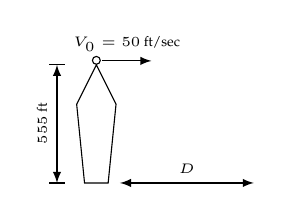
\begin{tikzpicture}
  \draw (0, 0) -- (.15, 0) -- (.25, 1) -- (0, 1.5) -- (-.25, 1) -- (-.15, 0) --
  cycle;
  \draw (0, 1.557) circle[radius = .05];
  \draw[latex-latex] (-.5, 0) -- (-.5, 1.5) node[pos = .5, font = \tiny,
  rotate = 90, above] {$555$ ft};
  \draw (-.6, 0) -- (-.4, 0);
  \draw (-.6, 1.5) -- (-.4, 1.5);
  \draw[-latex] (.075, 1.55) -- (.7, 1.55) node[pos = .5, above, font = \tiny]
  {$V_0 = 50$ ft/sec};
  \draw[latex-latex] (.3, 0) -- (2, 0) node[pos = .5, above, font = \tiny]
  {$D$};
\end{tikzpicture}
\end{document}
%%% Local Variables:
%%% mode: latex
%%% TeX-master: t
%%% End:
